Advances in processor efficiency along with the development of energy-harvesting systems have created a new category of devices that require neither a battery nor a tethered power supply~\cite{prasad_comst_2014,lucia_snapl_2017,soyata_csm_2016}. These devices operate using ambient energy, such as radio frequency transmissions~\cite{rf_powered_computing_gollakota_2014},
light~\cite{margolies_infocom_2016,margolies_tosn_2016}, and vibration~\cite{gorlatova_sigmetrics_2014}. Incorporating compute, storage, sensing, and communication hardware~\cite{wisp5,moo,capybara}, such devices are a promising technology for use in the Internet of Things~\cite{ku_cst_2016}, in-body~\cite{nadeau_naturebio_2017} and on-body~\cite{bandodkar_electroanalysis_2015} medical systems, and energy-harvesting nano-satellites~\cite{kicksat,capybara}. Energy-harvesting devices create unique challenges because they operate {\em intermittently} when energy is available~\cite{hicks_isca_2017,lucia_snapl_2017}. An energy-harvesting device buffers energy in a small storage capacitor~\cite{gorlatova_tmc_2013,gunduz_commag_2014} and operates when a threshold amount of energy has accumulated. Harvestable energy sources are low-power (e.g., \si{\nano\watt}\ to \si{\micro\watt}) compared to a platform's operating power level (hundreds of \si{\micro\watt}\ to \si{\milli\watt}). A device operates briefly until it depletes its buffered energy, after which, it shuts down and recharges to operate again later---corresponding to the {\em intermittent execution model}~\cite{dino,lucia_snapl_2017} composed of operation-power failure-restart cycles. The recharge and discharge intervals---which correspond to the device's inactive and active time---vary depending on the underlying hardware, such as the size of the energy buffering capacitor~\cite{capybara}, and some devices discharge and restart $\approx$10 to $\approx$100 times per second~\cite{tan_infocom_2016,mementos,nvp}.

Upon power failures, a device loses the volatile state in its registers, stack, SRAM, and retains the state of any non-volatile memory, such as FRAM. While capturing periodic checkpoints~\cite{mementos,quickrecall} and sleep scheduling~\cite{dewdrop,hibernus,hibernusplusplus} help preserve execution progress, failures can leave non-volatile state incorrect, partially updated, and may leave checkpointed volatile state inconsistent with non-volatile state. These inconsistencies cause intermittent execution to deviate from continuously-powered behavior, often leading to an unrecoverable application failure~\cite{dino,edb}. Prior work developed two main approaches to deal with data inconsistency for intermittently-powered devices: (i) \emph{software-based programming and execution models}~\cite{dino,ratchet,chain,alpaca} and (ii) \emph{hardware-based computer architecture support}~\cite{hicks_isca_2017,idetic,nvp}. Complex architectural changes are expensive to design, verify, and manufacture. New architectures are also inapplicable to existing systems~\cite{hicks_isca_2017,nvp}. Software approaches are simpler and applicable to existing devices today. \note{Talk about CP-based systems and talk why we focused task-based instead...}Therefore, this work focuses on a key limitation of task-based software approaches, that is, the {\em inflexibility} of statically decomposing a program into tasks.
%
\begin{figure}
    \centering
    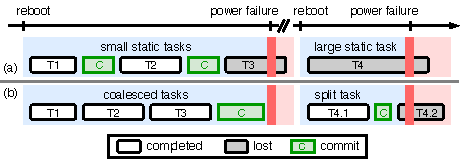
\includegraphics[width=\columnwidth]{figures/intro-figure-horiz.pdf}
    \caption{Task coalescing at runtime reduces time and energy overhead in task-based intermittent programming models by performing fewer commits (denoted as \texttt{C}) of individual tasks (denoted as \texttt{Tx}). On the other hand, task splitting reduces wasted computation and enables termination for bigger tasks.}
    \label{fig:coalesce}
\end{figure}
%
%\textbf{Task Decomposition of Intermittent Programs.} 
%
\textbf{Crucial Drawback of Static Task Decomposition.} Task-based programming and execution models require a programmer~\cite{alpaca,chain} or a compiler~\cite{baghsorkhi_cgo_2018} to statically decompose a program into a collection of tasks. A \emph{task}, a top level function, can include arbitrary computation that should be executed despite arbitrarily-timed power failures.
The programmer (or a compiler) explicitly expresses task-to-task control flow. Fig.~\ref{fig:coalesce} illustrates how a program's tasks execute and shows how tasks transitions can impose a runtime overhead. At each transition, the system incurs an overhead to track and atomically commit modifications to the non-volatile memory, to maintain consistency of program state~\cite{chain,alpaca}. The more task transitions a program requires, the more commit overhead is incurred by the system at runtime. A programmer may thus create very large tasks in an attempt to reduce task transitions overhead. However, a very large task may require more energy to complete than a device's fixed hardware energy buffer can hold which may lead to a task \emph{non-termination} problem. To eliminate this risk, existing systems require the programmer to decompose a program into relatively small tasks to preserve execution progress. These constraints on task sizing lead to the following dilemma: should large tasks be used, that are efficient but risk non-termination, or small tasks that are guaranteed to complete, but incur a high task transition and commit overhead. 

\textbf{Challenges and Contributions.} This paper introduces \sys, a new task-based system that employs \emph{adaptive task size execution by task coalescing/splitting}. By means of this novel technique, small tasks can be executed efficiently by trimming unnecessary overheads \emph{dynamically}, meanwhile avoiding the risk of non-termination. \sys accepts any static decomposition and it coalesces (groups) tasks (Fig.~\ref{fig:coalesce}, top) or splits them (Fig.~\ref{fig:coalesce},bottom) based on the estimated energy availability without demanding any hardware support. \note{\textbf{To the best of our knowledge, \sys is the only task-based system that guarantees task termination and ....(something related with Coalescing...)  }}

The unique challenges and contributions revealed by this work are listed below:
\note{it takes more space, but a bullet list makes C1-C3 stand out more properly}

% \sys does not requires hardware support for energy estimation to make its scheduling decisions. 

% \sys accepts any static decomposition and coalesces/splits its tasks at runtime. Two consecutive, coalesced tasks execute
% with no commit overhead between them, instead performing task-end commit actions at the end of the second task only.
% %
% When there is sufficient energy to execute both tasks, two distinct, small
% tasks are effectively executed as a single large task, preserving the atomicity
% of both. If power fails during a coalesced task, execution restarts from the
% {\em first} of the coalesced tasks. Figure~\ref{fig:coalesce} (top)
% illustrates how dynamic coalescing removes unnecessary overhead and shortens intermittent program execution.
% On the other hand, a large task that requires more energy to complete than a device buffered energy
% is split by \sys to enable task termination and preserve execution progress, as depicted in Figure~\ref{fig:coalesce} (bottom).

%\textbf{Challenges and Contributions} 
\noindent\note{Carlo's rephrasing} \emph{C1) Task Transition Overhead:} given unpredictable incoming energy, how to save progress as few times as possible? \sys tries to minimize task transition overhead by estimating energy conditions at run-time using \emph{recent execution history} as a metric.
% \noindent\emph{C1) Dynamic Task Sizing:} Given unpredictable energy shots arrival, how to specify the size of a dynamic task on the fly? \sys addresses this challenge by using a novel approach: \textit{recent execution history} as a metric to estimate the environment energy conditions and to specify task sizes. 
%Furthermore, It mitigates the risk of dynamic task re-execution by taking advantage of the certainty that the energy buffer offers and approaches the expected power interrupt carefully. 

\noindent\emph{C2) Dynamic Memory Consistency Handling:} merging static tasks on the fly gives rise to the need for dynamic memory consistency handling. How to dynamically detect inter-task data dependencies and ensure efficient protection against power interrupts? \sys does so by using a novel
approach called \emph{dynamic group privatization}--- %Varying variables dependencies forces a static approach (i.e.~\cite{alpaca}) to operate by considering a worst case scenario (i.e. protecting all global variables) in each dynamic task transition. 
performing real-time dependency tracking to enable protection on a task transition. Individual variables tracking, however, slows down a system dramatically. Therefore, \sys protects global variables in a batch. Moreover, it optimizes data transfers by using Direct Memory Access (DMA).

\noindent\emph{C3) Ensuring Task Termination:} a static task decomposition model assumes that each
single task can execute to completion. If the hardware energy buffer provides
inadequate energy to execute each single task to completion, a program will not
terminate~\cite{cleancut_2018}. Under such conditions, how to enable the dynamic execution model to progress on a sub-task level? To avoid non-termination under adverse
energy conditions, \sys uses a novel timer-based {\em partial task commit} mechanism \note{should we instead cite Ratchet?}.
Partial execution avoids non-termination by committing the intermediate state of a long-running
task that has repeatedly failed and restarted.
%Partial execution violates task atomicity, but preserves forward progress; if a programmer knows that task atomicity is crucial to correctness, they can disable partial execution around a piece of code.

%\begin{itemize}
%\item\textit{challenge} 1) Given unpredictable energy shots arrival, how to specify the size of a dynamic task on the fly? \textit{contribution---1} \sys addresses this challenge by using its \textit{recent execution history} as a metric to estimate the environment energy conditions. Furthermore, It mitigates the risk of dynamic task re-execution by taking advantage of the certainty that the energy buffer offers and approaches the expected power interrupt carefully. 
%%
%\item\textit{challenge} 2) Given dynamic variables dependencies, how to ensure efficient data protection against power interrupts? \textit{contribution---2} \sys ensures the consistency of the data by using a novel
%approach called \emph{dynamic group privatization}. Varying variables dependencies forces a static approach (i.e.~\cite{alpaca}) to operate by considering a worst case scenario (i.e. protecting all global variables) in each dynamic task transition. \sys, therefore, utilizes a real-time data tracking to enable partial data protection on a task transition. Individual variables tacking, however, slows down a system dramatically. Therefore, \sys  relies on a coarse locality principle and protects the global variables in a batch. Moreover, it optimizes the data transfer by using Direct Memory Access (DMA).
%%
%\item\textit{challenge} 3) A static task decomposition model assumes that each
%single task can execute to completion. If the hardware energy buffer provides
%inadequate energy to execute each single task to completion, a program will not
%terminate~\cite{cleancut_2018}. under such conditions how to enable the dynamic execution model to progress on a sub-task level? \textit{contribution---3} To avoid non-termination under adversarial
%energy conditions, \sys uses a timer-based {\em partial task commit} mechanism.
%Partial execution avoids non-termination by committing the intermediate state of a long-running
%task that has repeatedly failed and restarted. Partial execution violates
%task atomicity, but preserves forward progress; if a programmer knows that
%task atomicity is crucial to correctness, they can disable partial execution around a piece of code.
%\end{itemize}
%

To asses the benefits of \sys over existing task-based systems, we implemented and tested six
benchmarks on a real energy-harvesting platform.
Our evaluation shows that \sys reduces run time by up to 54\%, and by 26\% on average, as compared to a state-of-the-art system, and is able to progress where static systems fail.
 
The rest of this paper is organized as follows. Section~\ref{sec:background} provides background on intermittent computing.
Section~\ref{sec:systemdescription} provides an overview of \sys, while
Section~\ref{sec:task_adaptation} describes \sys's energy-adaptive mechanism. The dynamic group privatization is explained in Section~\ref{sec:memory_virtulaization}. Implementation details of \sys are given in Section~\ref{sec:implementation}. Sections~\ref{sec:methodology} and~\ref{sec:evaluation} describe \sys's evaluation methodology and results. Section~\ref{sec:related_work} positions \sys in the
context of related work and Section~\ref{sec:conclusions} concludes and discusses
future work.
